% Symbol Table Implementation - Formal Book-style Chapter
% Suitable for Overleaf
\documentclass[11pt,a4paper]{book}
\usepackage[utf8]{inputenc}
\usepackage{lmodern}
\usepackage{microtype}
\usepackage{amsmath,amssymb}
\usepackage{graphicx}
\usepackage{tikz}
\usetikzlibrary{shapes,arrows.meta,positioning,decorations.pathmorphing}
\usepackage{hyperref}
\usepackage{longtable}
\usepackage{caption}
\usepackage{listings}
\usepackage{color}

% Listings style for small C snippets
\definecolor{codegray}{rgb}{0.95,0.95,0.95}
\lstset{backgroundcolor=\color{codegray},basicstyle=\ttfamily\small,breaklines=true}

\title{Symbol Table Implementation\newline\large A Formal Explanation with Diagrams}
\author{Compiler Design Laboratory}
\date{}

\begin{document}

\maketitle
\tableofcontents
\cleardoublepage

\chapter{Introduction}

This chapter provides a formal, book-style description of a production-grade symbol-table implementation used in a C-like compiler. The implementation combines two complementary data structures: a hash table for fast name-based lookup and a doubly-linked global list for ordered traversal and scope-management operations. The design goals of the implementation are:

\begin{itemize}
  \item Provide O(1) average-time symbol lookup.
  \item Maintain insertion order for readable printing and deterministic iteration.
  \item Support nested scopes, shadowing, and safe deletion of symbols upon scope exit.
  \item Provide a compact type abstraction (base types, pointer types, array types) to facilitate type-checking.
\end{itemize}

The following sections present the API, data structures, algorithms, and examples, together with precise diagrams implemented using Ti\textit{k}Z so the document can be compiled on Overleaf.

\chapter{Data Types and Structures}

\section{Data Type Enumeration}

The implementation models types using an enumerated set. The enumeration provides a clear and compact representation of base types, pointer types and array types.

\begin{lstlisting}[language=C]
typedef enum {
    TYPE_INT,
    TYPE_FLOAT,
    TYPE_CHAR,
    TYPE_VOID,
    TYPE_UNKNOWN,
    TYPE_INT_PTR,
    TYPE_FLOAT_PTR,
    TYPE_CHAR_PTR,
    TYPE_INT_ARRAY,
    TYPE_FLOAT_ARRAY,
    TYPE_CHAR_ARRAY
} data_type_t;
\end{lstlisting}

Each symbol's type is represented by a value of type \texttt{data\_type\_t}. Pointers and arrays are distinct enum values to simplify semantic checks (e.g., base-type extraction).

\section{Scope Types}

Scopes are classified into three categories:

\begin{lstlisting}[language=C]
typedef enum {
    SCOPE_GLOBAL,
    SCOPE_FUNCTION,
    SCOPE_BLOCK
} scope_type_t;
\end{lstlisting}

In addition to this categorical classification, the symbol table tracks an integer \emph{scope level} representing nesting depth (0 for global, 1 for the first nested block, and so on).

\section{Symbol Node Structure}

The core storage unit is the symbol node. Each node stores identifying information, type and scope metadata, and pointers used by the two linking structures (hash chain and global doubly-linked list).

\begin{lstlisting}[language=C]
typedef struct symbol_node {
    char name[MAX_ID_LENGTH];
    data_type_t type;
    scope_type_t scope;
    int scope_level;
    int line_declared;
    int is_function;
    int is_array;
    int array_size;
    int is_pointer;
    struct symbol_node* hash_next; // chain in hash bucket
    struct symbol_node* next;      // global linked list next
    struct symbol_node* prev;      // global linked list prev
} symbol_node_t;
\end{lstlisting}

Two linked structures are used simultaneously:

\begin{itemize}
  \item Hash chaining via \texttt{hash\_next} for O(1) expected lookup.
  \item A global doubly-linked list via \texttt{next} and \texttt{prev} to preserve insertion order and permit O(1) deletion when a node pointer is known.
\end{itemize}

\section{Symbol Table Container}

The global symbol table structure aggregates the hash table and the doubly-linked list heads and metadata:

\begin{lstlisting}[language=C]
typedef struct {
    symbol_node_t* hash_table[HASH_TABLE_SIZE];
    symbol_node_t* head; // global list head
    symbol_node_t* tail; // global list tail
    int count;
    int current_scope_level;
} symbol_table_t;
\end{lstlisting}

\chapter{Hashing and Initialization}

\section{Hash Function}

A DJB2-inspired hash is used to map identifier names to bucket indices. The algorithm uses a seed value and multiplies by 33 on each step, which yields a simple, fast hash with good empirical distribution for short identifiers.

\begin{lstlisting}[language=C]
unsigned int hash(const char* name) {
    unsigned int hash_value = 5381;
    int c;
    while ((c = *name++)) {
        hash_value = ((hash_value << 5) + hash_value) + c; // hash * 33 + c
    }
    return hash_value % HASH_TABLE_SIZE;
}
\end{lstlisting}

The result is reduced modulo a prime table size (the implementation uses 211) to lower clustering and achieve a better spread of identifiers across buckets.

\section{Initialization}

The symbol table is initialized by setting every hash bucket to \texttt{NULL}, clearing the global list heads, resetting the symbol count and setting the current scope level to 0.

\begin{lstlisting}[language=C]
void init_symbol_table() {
    for (int i = 0; i < HASH_TABLE_SIZE; i++)
        sym_table.hash_table[i] = NULL;
    sym_table.head = NULL;
    sym_table.tail = NULL;
    sym_table.count = 0;
    sym_table.current_scope_level = 0;
}
\end{lstlisting}

\chapter{Insertion and Duplicate Detection}

\section{Duplicate Detection: Scope-aware}

A symbol may be redeclared in an inner scope (shadowing), which is allowed, but redeclaration in the same scope is an error. To enforce this rule the implementation provides a function that looks up a name in a specific scope level only.

\begin{lstlisting}[language=C]
symbol_node_t* lookup_symbol_in_scope(char* name, int scope_level) {
    unsigned int hash_index = hash(name);
    symbol_node_t* current = sym_table.hash_table[hash_index];
    while (current != NULL) {
        if (strcmp(current->name, name) == 0 && current->scope_level == scope_level)
            return current;
        current = current->hash_next;
    }
    return NULL;
}
\end{lstlisting}

When adding a new symbol, the code calls \texttt{lookup\_symbol\_in\_scope()} for the \texttt{sym\_table.current\_scope\_level}. If a match is found, insertion is rejected and an error is produced with the line number of the prior declaration.

\section{Adding a Symbol (full form)}

The full insertion routine (which supports arrays, pointers and functions) performs the following steps:

\begin{enumerate}
  \item Check for duplicate in the same scope using \texttt{lookup\_symbol\_in\_scope}. If found, return failure.
  \item Allocate a new \texttt{symbol\_node\_t} and populate its fields (name, type, flags, scope information and initialize internal pointers to NULL).
  \item Insert the new node at the head of the corresponding hash bucket (prepending) to achieve O(1) insertion.
  \item Append the new node to the global doubly-linked list (tail insertion) to preserve declaration order.
  \item Increment the symbol count and optionally print a debug message.
\end{enumerate}

This combination of prepending to the hash chain and appending to the global list yields efficient lookup and predictable iteration order.

\chapter{Lookup and Scope Resolution}

\section{Lookup Algorithm}

Lookup is hash-based, but scope-aware: given an identifier name the code locates the bucket using the hash, then searches the bucket's chain, preferring the innermost (current) scope and falling back to outer scopes.

Pseudo-procedure:

\begin{enumerate}
  \item Compute bucket index by hashing the name.
  \item For level = current\_scope\_level down to 0:\newline
    \quad traverse the bucket chain and return the first node whose name matches and whose \texttt{scope\_level} equals the current tested level.
  \item If not found at any level, return \texttt{NULL}.
\end{enumerate}

This ensures correct shadowing behavior: an inner scope's declaration masks an outer one during lookup.

\begin{lstlisting}[language=C]
symbol_node_t* lookup_symbol(char* name) {
    unsigned int hash_index = hash(name);
    symbol_node_t* current = sym_table.hash_table[hash_index];
    for (int level = sym_table.current_scope_level; level >= 0; level--) {
        symbol_node_t* temp = current;
        while (temp != NULL) {
            if (strcmp(temp->name, name) == 0 && temp->scope_level == level)
                return temp;
            temp = temp->hash_next;
        }
    }
    return NULL;
}
\end{lstlisting}

\chapter{Scope Management: Entering and Exiting Scopes}

\section{Entering a Scope}

Entering a new block increments the \texttt{current\_scope\_level}. This is typically invoked when the parser recognizes a left brace ('{').

\begin{lstlisting}[language=C]
void enter_scope() {
    sym_table.current_scope_level++;
}
\end{lstlisting}

\section{Exiting a Scope}

Exiting a scope requires removing all symbols declared at the exiting scope level. The implemented strategy traverses the global doubly-linked list and removes any node whose \texttt{scope\_level} equals the current scope. For each node to be removed the following actions are taken:

\begin{enumerate}
  \item Unlink the node from its hash chain by scanning the bucket chain and patching links.
  \item Unlink the node from the global doubly-linked list by updating the \texttt{prev}'s \texttt{next} and the \texttt{next}'s \texttt{prev} pointers (handling head/tail cases explicitly).
  \item Free the node's memory and decrement the symbol count.
\end{enumerate}

After removing all relevant entries, the scope level is decremented (with a floor at 0 to avoid underflow).

\begin{lstlisting}[language=C]
void exit_scope() {
    symbol_node_t* current = sym_table.head;
    while (current != NULL) {
        symbol_node_t* next_node = current->next; // saved before possible deletion
        if (current->scope_level == sym_table.current_scope_level) {
            // remove from hash bucket chain (scan and patch)
            // remove from global doubly-linked list (handle head/tail)
            // free(current); sym_table.count--;
        }
        current = next_node;
    }
    if (sym_table.current_scope_level > 0)
        sym_table.current_scope_level--;
}
\end{lstlisting}

This approach is simple and safe. A possible improvement is to maintain an explicit per-scope list of nodes so that exit becomes proportional only to the number of symbols in that scope rather than the total number of symbols.

\chapter{Printing and Introspection}

A formatted printer walks the global doubly-linked list from \texttt{head} to \texttt{tail} and prints a table containing: name, type (string), scope category (string), scope level, declaration line, function flag and array/pointer info.

\begin{lstlisting}[language=C]
void print_symbol_table() {
    symbol_node_t* current = sym_table.head;
    while (current != NULL) {
        // format and print fields
        current = current->next;
    }
}
\end{lstlisting}

Because the global list preserves insertion order, the printed table reflects the original declaration order, which improves human readability during debugging and grading.

\chapter{Type Utilities and Compatibility}

The implementation includes utility routines that convert enum types to human-readable strings and helpers that obtain the base type from pointers/arrays. These utilities simplify the type checking logic.

\begin{lstlisting}[language=C]
char* type_to_string(data_type_t type) { /* returns "int", "float", "int*" etc. */ }
char* scope_to_string(scope_type_t scope) { /* returns "global", "function", "block" */ }
\end{lstlisting}

Type compatibility is determined by a small set of rules:

\begin{itemize}
  \item Exact-type equality is compatible.
  \item Integer and char are treated as compatible (integer promotion).
  \item Float is compatible only with float.
  \item Pointer and array types are compatible through their base type (arrays decay to pointers for many checks).
\end{itemize}

A representative implementation:

\begin{lstlisting}[language=C]
int are_types_compatible(data_type_t type1, data_type_t type2) {
    if (type1 == type2) return 1;
    data_type_t base1 = get_base_type(type1);
    data_type_t base2 = get_base_type(type2);
    if ((base1 == TYPE_INT || base1 == TYPE_CHAR) &&
        (base2 == TYPE_INT || base2 == TYPE_CHAR)) return 1;
    if (base1 == TYPE_FLOAT && base2 == TYPE_FLOAT) return 1;
    return 0;
}
\end{lstlisting}

\chapter{Key Algorithms and Complexity}

\section{Time Complexity}

\begin{description}
  \item[add\_symbol:] Average O(1) (prepend to hash chain), worst-case O(n) if all names collide.
  \item[lookup\_symbol:] Average O(1), worst-case O(n) per lookup when collision chain degenerates.
  \item[exit\_scope:] O(n) in the current implementation since it scans the global list to find nodes belonging to the exiting scope.
  \item[print\_symbol\_table:] O(n) for full traversal.
\end{description}

\section{Space Complexity}

Total space is O(n + m), where n is the number of symbols and m is the hash-table size (211). Each symbol node stores fixed-size fields and three pointers; on a 64-bit platform a node size is on the order of a few dozen bytes plus the identifier buffer.

\chapter{Diagrams}

The following diagrams illustrate the data structures and relationships. They are implemented with Ti\textit{k}Z so they render natively in PDF output.

\section{Symbol Node Layout}

\begin{center}
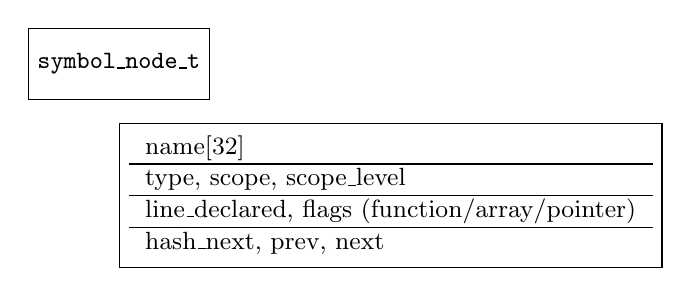
\begin{tikzpicture}[node distance=6mm, every node/.style={font=\small}]
  \node[draw,rectangle,minimum height=9mm] (node) {\texttt{symbol\_node\_t}};
  \node[draw,rectangle,below=3mm of node,minimum height=6mm,anchor=north west] (fields) {
    \begin{tabular}{l}
    name[32] \\\hline
    type, scope, scope\_level \\\hline
    line\_declared, flags (function/array/pointer) \\\hline
    hash\_next, prev, next
    \end{tabular}
  };
\end{tikzpicture}
\end{center}

\section{Hash Table with Chaining}

\begin{center}
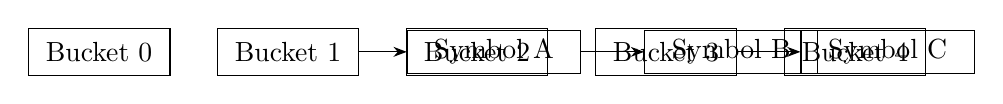
\begin{tikzpicture}[node distance=8mm, >=Stealth]
  % Buckets
  \foreach \i in {0,1,2,3,4} {
    \node[draw,rectangle,minimum width=18mm,minimum height=6mm] (b\i) at (\i*2.4,0) {Bucket \i};
  }
  % Chains
  \node[draw,rectangle,minimum width=22mm,right=6mm of b1] (sA) {Symbol A};
  \node[draw,rectangle,minimum width=22mm,right=8mm of sA] (sB) {Symbol B};
  \node[draw,rectangle,minimum width=22mm,right=8mm of b3] (sC) {Symbol C};

  \draw[->] (b1) -- (sA);
  \draw[->] (sA) -- (sB);
  \draw[->] (b3) -- (sC);
\end{tikzpicture}
\end{center}

\section{Global Doubly-Linked List}

\begin{center}
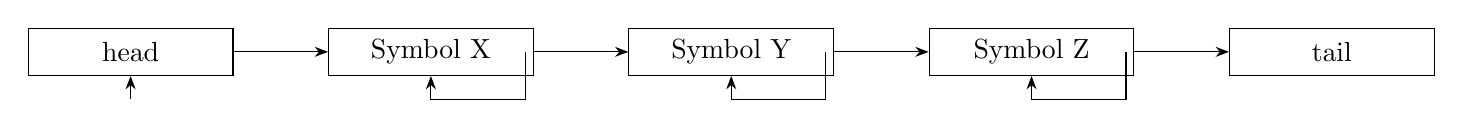
\begin{tikzpicture}[node distance=12mm, >=Stealth, every node/.style={draw,rectangle,minimum width=26mm,minimum height=6mm}]
  \node (h) {head};
  \node[right=12mm of h] (n1) {Symbol X};
  \node[right=12mm of n1] (n2) {Symbol Y};
  \node[right=12mm of n2] (n3) {Symbol Z};
  \node[right=12mm of n3] (t) {tail};

  \draw[->] (h) -- (n1);
  \draw[->] (n1) -- (n2);
  \draw[->] (n2) -- (n3);
  \draw[->] (n3) -- (t);

  \draw[<-] (h) -- ++(0,-6mm);
  \draw[<-] (n1) -- ++(0,-6mm) -- ++(12mm,0) -- ++(0,6mm) ;
  \draw[<-] (n2) -- ++(0,-6mm) -- ++(12mm,0) -- ++(0,6mm) ;
  \draw[<-] (n3) -- ++(0,-6mm) -- ++(12mm,0) -- ++(0,6mm) ;
\end{tikzpicture}
\end{center}

\chapter{Examples and Use Cases}

\section{Simple Declaration}

A top-level declaration such as \texttt{int x;} results in a single symbol node inserted into the hash table and appended to the global list. If the identifier hashes to bucket 120 it will appear at the head of that bucket's chain and at the tail of the global list.

\section{Nested Scopes and Shadowing}

The lookup algorithm searches from the current scope level outward. Consider:

\begin{verbatim}
int x;      // level 0
{
  int x;    // level 1, shadows outer x
  // lookup("x") returns the level-1 symbol
}
// lookup("x") now returns the level-0 symbol
\end{verbatim}

\chapter{Potential Improvements}

We highlight several low-risk, high-value improvements:

\begin{itemize}
  \item Maintain a per-scope stack of symbols: this makes \texttt{exit\_scope} proportional only to the number of symbols declared in that scope rather than the global symbol count.
  \item Dynamic resizing of the hash table: resize when the load factor exceeds a threshold to keep averages close to O(1).
  \item String interning for identifier names to reduce memory usage and speed up string comparisons by pointer equality.
  \item Separate the type system into an independent module to improve modularity and testability of type checking rules.
\end{itemize}

\chapter{Conclusion}

The presented hybrid symbol-table design balances lookup performance and iteration semantics. It is simple to implement, easy to reason about, and suitable for teaching and for small-to-medium compiler projects. The design handles shadowing, supports a compact set of types, and provides clear hooks for future extensions such as per-scope lists and dynamic hash resizing.

\appendix
\chapter{How to Use this File on Overleaf or Locally}

To use this file on Overleaf, upload \texttt{symbol\_table.tex} to a new Overleaf project, and compile. Overleaf natively supports Ti\textit{k}Z.

To compile locally using \texttt{pdflatex}:

\begin{verbatim}
pdflatex symbol_table.tex
pdflatex symbol_table.tex
\end{verbatim}

(Repeat twice to ensure the table of contents and references are resolved.)

\chapter{Acknowledgements}

This chapter formalizes and re-styles an educational symbol table implementation used in the Compiler Design Laboratory exercises; diagrams and exposition are adapted to a textbook-style presentation.

\end{document}
